\documentclass[10pt,twocolumn,letterpaper]{article}
\usepackage[margin=.75in]{geometry}
\usepackage[T1]{fontenc}
\usepackage{courier}
\usepackage{newtxtext,amsmath,amssymb,graphicx,booktabs,natbib}
\usepackage[hyphens]{url}
\sloppy
\title{Candidate Quality and Delivered Accuracy Can Move in Opposite Directions}
\author{}\date{}
\begin{document}\maketitle
\begin{abstract}An evidence-only planner adds four correct deliveries but two wrong deliveries on 96 TAT-QA contexts, while correct candidates decrease 26 to 25. It therefore fails its practical adoption rule despite conditional recovery in answer-key diagnostics. A secondary comparison gives no delivery gain. This short report separates candidate generation from selective delivery and retains resource, scoring and statistical qualifications.\end{abstract}

\section{Question and Scope}
Can an evidence-only planner realize the recovery suggested by answer-key diagnostic interventions? We examine this question in completed financial program-generation experiments. Our contribution is a failure analysis of specific local recipes, not a new winning algorithm. Financial programs can execute correctly while selecting the wrong period, row, unit or operation. A verifier can also reduce wrong delivery by withholding most answers. Candidate construction and delivered correctness must therefore remain distinct.

\section{Design and Measurements}
The planning comparison uses four completed arms on 96 project-held-out TAT-QA contexts: direct 7B, program-generating 7B, a smaller multi-role pipeline (MAS), and planner MAS. Models belong to Qwen2.5; the full record specifies model hashes, adapters, prompts and decoding \citep{qwen}. Evidence packets do not expose answer labels. Programs refer to source quantities and arithmetic steps; deterministic execution establishes arithmetic/provenance constraints, not financial semantic validity. The planner predicts operations, dependencies and VALUE placeholders from question/evidence without answer-key supervision. Its token allocation also changes the actor budget, so this is a pipeline intervention rather than an isolated planning-stage causal effect.

Let $K_i$ indicate a correct executable candidate and $D_i$ delivery. Correct delivery is $n^{-1}\sum_i K_iD_i$; wrong delivery is $n^{-1}\sum_i(1-K_i)D_i$. Withholding is $n^{-1}\sum_i(1-D_i)$. These observables distinguish generation from acceptance \citep{selective}. The prespecified practical requirement combines a positive paired correct-delivery interval with no observed increase in wrong delivery. A secondary 28-context cohort tests the direction again.

The Windows experiment is a nominal 8 GB \emph{application-budget tier} on a 16.39 GB host. A 6.1 GB worker commit ceiling and sampled working-set guard do not establish physical 8 GB feasibility or absence of paging. Greedy single-seed runs do not measure training/decoding variation. FinQA and arithmetic TAT-QA are public financial reasoning benchmarks \citep{finqa,tatqa}; project-held-out filtering does not exclude pretraining contamination.

\section{Results: Recovery Does Not Establish Improvement}
\begin{figure*}[t]\centering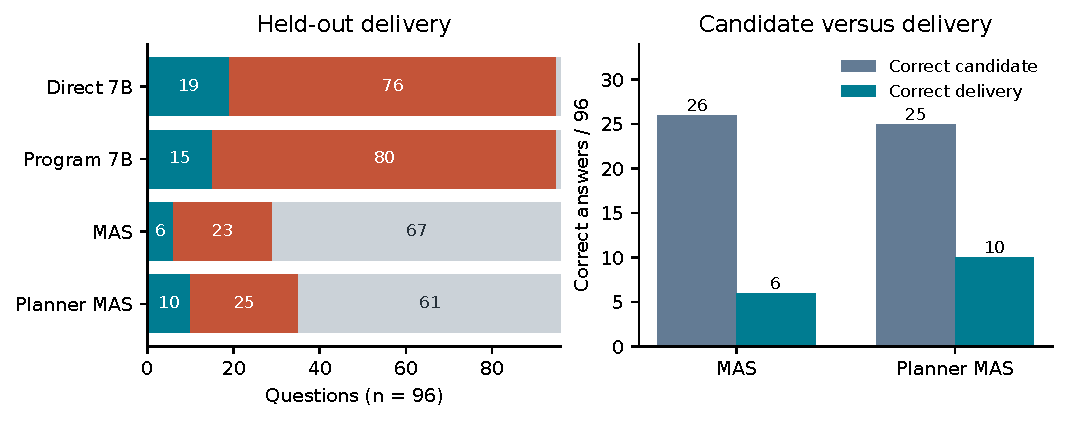
\includegraphics[width=.80\textwidth]{figures/planner_outcomes.pdf}\caption{All 96-context arms: delivered outcomes and correct candidates. Planner delivery gains coexist with lower correct-candidate count.}\label{tab:planner}\end{figure*}
The planner gains four correct deliveries and loses none, but adds two wrong deliveries (Figure~\ref{tab:planner}). The correct-delivery change is $+4.2$ percentage points, with paired context-bootstrap 95\% interval approximately $[+1.0,+8.3]$; exact paired $p=0.125$. Sparse discordant pairs and the bootstrap/exact-test disagreement preclude an established accuracy improvement. More importantly, the practical conjunction fails because wrong delivery increases. Correct executable candidates decrease from 26 to 25: the delivered gain is not a net generation gain.

On the secondary 28-context cohort both MAS arms deliver 2 correct, 10 wrong and withhold 16; correct candidates decrease 5 to 3. The attempted 7B comparison stops after a two-context prefix because of allocation failure, leaving that baseline incomplete. Planner median resident request time rises 25.2 to 33.9 seconds; generated tokens rise 6672 to 9863. Commit remains about 5.26 GB. Cross-arm direct/program timings include model loading and are not matched resident-latency comparisons.

The oracle diagnostic supplies reference operation structure and an operand shortlist on 15 enriched FinQA cases. Official execution matches change 0/0/4/10 across neither/operands/structure/both. These answer-key inputs supply unavailable solution information and are neither a deployable planner nor a universal reasoning upper bound. Even the combined intervention yields only 7 reported-answer matches; numerical scoring conventions are not interchangeable.

\section{Boundary Conditions and Implications}
The complementary 160-question FinQA deployment study yields 78/48/34 reported C/W/H for a 14B quantized recipe versus 5/3/152 for a resident F16 team; raw scoring changes the first arm to 38/88/34. Model size, precision, pipeline and runtime differ, so the studies cannot establish a pure architectural effect. Stronger direct baselines, null precision/retrieval/repair results and a favorable cache-only memory change remain in the full support, not independent confirmations of the planner.

The defensible implication is to measure evidence availability, candidate correctness, wrong/correct delivery and resource cost separately. Sparse gains, model/prompt dependence, missing TAT-QA report clusters, public-data exposure and incomplete baselines limit generality. No professional financial validity or autonomous-deployment safety follows.

\section{Conclusion}
The planner fails its practical criterion. Four additional correct deliveries do not establish a generation gain when correct candidates decrease and wrong delivery increases. Oracle recoverability and deployable improvement must remain distinct.
\section*{Support and AI Assistance}
The accompanying 29-page audited supplement preserves complete methods, all cohorts, historical outcomes, statistical derivations and examples. Codex assisted this adaptation and code-based checks of preserved evidence; no new inference was run. Human authors must review correctness, originality, declarations and destination-specific rules before submission. This generic draft is not certified for any named workshop.
\bibliographystyle{plainnat}\bibliography{references}
\end{document}
